\documentclass[a4paper,11pt]{article}
\usepackage[top=2cm,bottom=2cm,left=2cm,right=2cm]{geometry}
\usepackage[utf8]{inputenc}
\usepackage[frenchb]{babel}

\usepackage{multirow}
\usepackage{makecell}
\usepackage{fancyhdr}
\usepackage{caption}
\usepackage[final]{pdfpages}
\usepackage{tikz,pgfplots,pgf}
\usepackage{subcaption}
\usepackage{siunitx}
\usepackage[toc,page]{appendix}
\usepackage{tcolorbox, listings} 
\usepackage{sectsty}
\usepackage[french]{minitoc} 
\usepackage{hyperref}
\usepackage{colortbl}
\usepackage{mwe}
\usepackage{amsmath}
\usepackage{lipsum}
\usepackage{enumitem}

\definecolor{Pantone2377C}{HTML}{2C5574}
\definecolor{subtitlecolour}{HTML}{00A2A9}
\definecolor{codegreen}{rgb}{0,0.6,0}
\definecolor{codegray}{rgb}{0.5,0.5,0.5}
\definecolor{codeblue}{HTML}{3E8BC0}
\definecolor{codeorange}{HTML}{ffa334}
\definecolor{backcolour}{HTML}{efefef}

\lstdefinestyle{myPython}{
    language=Python,
    backgroundcolor=\color{backcolour},   
    commentstyle=\color{codegreen},
    otherkeywords={plt, np, df},
    keywordstyle=\color{codeblue},
    numberstyle=\tiny\color{codegray},
    stringstyle=\color{codeorange},
    basicstyle=\ttfamily\footnotesize,
    breakatwhitespace=false,         
    breaklines=true,                 
    keepspaces=true,                 
    numbers=left,       
    numbersep=5pt,                  
    showspaces=false,                
    showstringspaces=false,
    showtabs=false,                  
    tabsize=2,
    inputencoding=utf8
}

\lstdefinestyle{myLog}{
    backgroundcolor=\color{backcolour},   
    basicstyle=\ttfamily\footnotesize,
    breakatwhitespace=false,         
    breaklines=true,                 
    keepspaces=true,                 
    numbers=left,       
    numbersep=5pt,                  
    showspaces=false,                
    showstringspaces=false,
    showtabs=false,                  
    tabsize=2,
    inputencoding=utf8
}

\lstset{
  backgroundcolor=\color{backgroundColour},   
  commentstyle=\color{codegreen},
  keywordstyle=\color{codeblue},
  numberstyle=\tiny\color{codegray},
  stringstyle=\color{codeorange},
  basicstyle=\footnotesize,
  breakatwhitespace=false,         
  breaklines=true,                 
  captionpos=b,                    
  keepspaces=true,                 
  numbers=left,                    
  numbersep=5pt,                  
  showspaces=false,                
  showstringspaces=false,
  showtabs=false,                  
  tabsize=2,
  literate=
  {é}{{\'e}}1
  {è}{{\`{e}}}1
  {ê}{{\^{e}}}1
  {û}{{\^{u}}}1
  {ù}{{\`{u}}}1
  {â}{{\^{a}}}1
  {à}{{\`{a}}}1
  {ç}{{\c{c}}}1
  {Ç}{{\c{C}}}1
  {ô}{{\^{o}}}1
}

\hypersetup{
	colorlinks=true, %colorise les liens
	breaklinks=true, %permet le retour à la ligne dans les liens trop longs
	urlcolor= blue,  %couleur des hyperliens
	linkcolor= black, %couleur des liens internes
	plainpages=false  %pour palier à "Bookmark problems can occur when you have duplicate page numbers, for example, if you have a page i and a page 1."
}

% Entête et pied de page
\pagestyle{fancy}
\rhead{
\includegraphics [scale=0.035]{img/ensta-logo.png}}
\chead{}
\lhead{}
\lfoot{Tanguy ROUDAUT - Tadios QUINIO}
\rfoot{FIPA promotion 2024}
\cfoot{\thepage}
\renewcommand{\headrulewidth}{0.4pt}
\renewcommand{\footrulewidth}{0.4pt}


\title{TP5: Tests du $\chi^{2}$ sur une distribution d’un échantillon}
\author{Tanguy ROUDAUT — Tadios QUINIO \and FIPASE 24}
\date{11 Octobre 2022}

\begin{document}

\maketitle

\vspace{1cm}
\section{Retrouver la loi}
\vspace{.2cm}

\noindent
À l’aide de 100 antennes GPS, en des points différents du globe\footnote{Éventuellement dans des environnements fortement métalliques ou partiellement enterrés}, le nombre de satellites visibles a été
compté :

\begin{center}
    \begin{tabular}{| c | c | c | c | c | c | c | c | c | c |}
        \hline
        Nombre de satellites & 1 & 2 & 3 & 4 & 5 & 6 & 7 & 8 & 9  \\ \hline
        Nombre d’observations & 6 & 15 & 9 & 25 & 17 & 10 & 8 & 7 & 3 \\ \hline
    \end{tabular}
\end{center}


%%%%%
\vspace{.5cm}
\begin{itemize}[label={},itemindent=-2em,leftmargin=2em]
    \item \textbf{Question~1~:} Estimer la moyenne et la variance de l’échantillon. Indication: on utilisera les opéra-
    teurs terme à terme python: \textit{**} et \textit{*}?
\end{itemize}
\vspace{.2cm}

\noindent
Formules utilisées~:

\begin{figure}[!h]
    \centering
    \begin{minipage}{.48\linewidth}
        \begin{equation}
            \overline{x}_{n} = \frac{\sum{(n_{i}.x_{i})}}{n}
        \end{equation}
    \end{minipage}\hfill\vline
    \begin{minipage}{.48\linewidth}
        \begin{equation}
            S^{2}_{n-1} = \frac{1}{n-1} \sum^{k}_{k=1}{n_{k}.(x_{k}-\overline{x}_{n})^{2}}
        \end{equation}
    \end{minipage}
\end{figure}



\begin{lstlisting}[style=myPython, caption=Code Python question 1, frame=lines]
obs = np.array([6, 15, 9, 25, 17, 10, 8, 7, 3])
sat = np.array([1, 2, 3, 4, 5, 6, 7, 8, 9])

nObs = 0
nSat = 0
for i in range(len(obs)):
    nObs += obs[i]
    nSat += sat[i]

num_mean = 0
for i in range(len(obs)):
    num_mean += obs[i]*sat[i]
mean = num_mean / nObs

num_var = 0
for i in range(len(obs)):
    num_var += (sat[i]-mean)**2
var = num_var/(len(sat)-1)

print("Question 1:")
print(" Moyenne =", mean)
print(' Variance =', var, end="\n\n")    
\end{lstlisting}

\begin{lstlisting}[style=myLog, caption=Résultat du code, frame=lines]
Question 1:
    Moyenne = 4.47
    Variance = 7.816012499999999
\end{lstlisting}

%%%%%
\vspace{.5cm}
\begin{itemize}[label={},itemindent=-2em,leftmargin=2em]
    \item \textbf{Question~2~:} Approcher la loi sous-jacente à l’aide d’une loi de Poisson de paramètre $\lambda = 4.47$. Déter-
    miner les effectifs théoriques pour 0 à 16 satellites. Indication: on utilisera la fonction \textit{poisson.pmf}.
\end{itemize}
\vspace{.2cm}

Grâce au code python ci-dessous, nous avons obtenus les effectifs théoriques suivants pour les satellites visibles de 0 à 16~:

\vspace{.1cm}

\begin{figure}[!h]
    \centering
    \begin{minipage}{.42\linewidth}
        \begin{center}
            \begin{tabular}{| c | c | c | c |}
                \hline
                \multicolumn{2}{|c|}{\textbf{Donnés}} & \multicolumn{2}{|c|}{\textbf{Estimés}} \\ \hline
                \textbf{Nb sat} & \textbf{Nb d'obs} & \textbf{Proba} & \textbf{eff th} \\ \hline\hline
                0 & N.C & 0.011 & 1.145 \\ \hline\hline
                1 & 6 & 0.051 & 5.117 \\ 
                2 & 15 & 0.114 & 11.436 \\ 
                3 & 9 & 0.17 & 17.04 \\ 
                4 & 25 & 0.19 & 19.042 \\
                5 & 17 & 0.17 & 17.024 \\ 
                6 & 10 & 0.127 & 12.683 \\ 
                7 & 8 & 0.081 & 8.099 \\ 
                8 & 7 & 0.045 & 4.525 \\ 
                9 & 3 & 0.022 & 2.248 \\ \hline\hline
                10 & N.C & 0.01 & 1.005 \\ 
                11 & N.C & 0.004 & 0.408 \\ 
                12 & N.C & 0.002 & 0.152 \\ 
                13 & N.C & 0.001 & 0.052 \\ 
                14 & N.C & 0.0 & 0.017 \\ 
                15 & N.C & 0.0 & 0.005 \\ 
                16 & N.C & 0.0 & 0.001 \\ \hline
            \end{tabular}
        \end{center}
    \end{minipage}\hfill
    \begin{minipage}{.54\linewidth}
        \begin{center}
            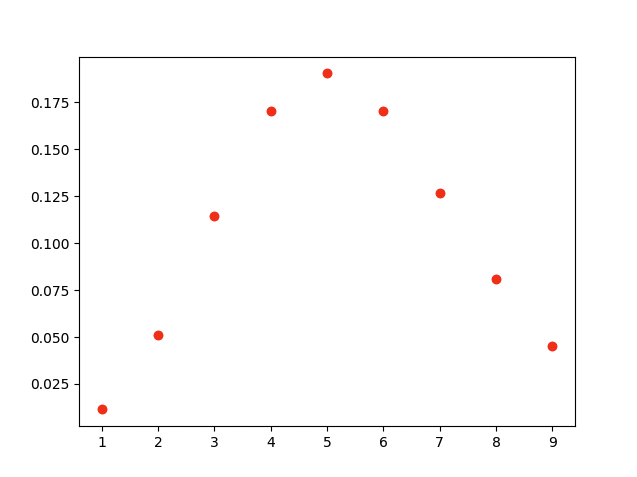
\includegraphics[width=1\textwidth]{img/figure1.png}
            \caption{\label{fig:figure1}Loi sous-jacente approcher par une loi de Poisson pour 1 à 9~satellites}

            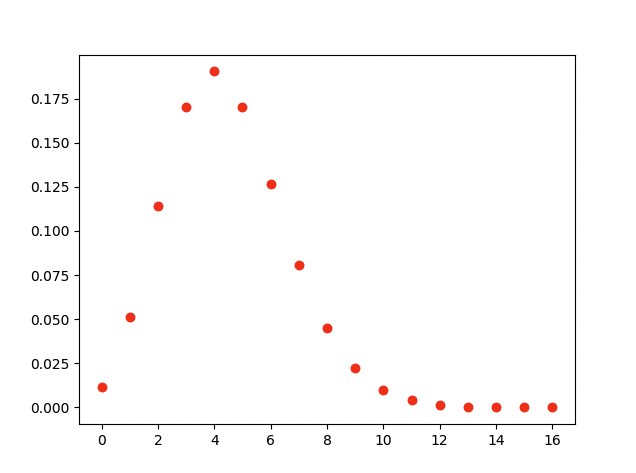
\includegraphics[width=1\textwidth]{img/figure2.png}
            \caption{\label{fig:figure1}Loi sous-jacente approcher par une loi de Poisson pour 0 à 16~satellites}
        \end{center}
    \end{minipage}
\end{figure}


\vspace{.1cm}

\begin{lstlisting}[style=myPython, caption=Code Python question 2, frame=lines]
Lambda = 4.47
poisson_array = np.zeros((17,))
effectifs_th = np.zeros((17,))
print("Question 2:")
print("nb Sat |  nb Obs  |  Proba  |   eff th")
print("=========================================")
poisson_array[0] = stats.poisson.pmf(0, Lambda)
effectifs_th[0] = nObs * poisson_array[0]
print("  ", 0, "  |  ", "N.C", "  |\t", round(poisson_array[0], 3), "\t|\t", round(effectifs_th[0], 3))
print("-----------------------------------------")

for i in range(1, len(sat)+1):
    poisson_array[i] = stats.poisson.pmf(sat[i-1], Lambda)
    effectifs_th[i] = nObs * poisson_array[i]

    print("  ", sat[i-1], "  |   ", round(obs[i-1], 2), "\t |\t", round(poisson_array[i], 3), "\t|\t", round(effectifs_th[i], 3))

print("-----------------------------------------")

plt.plot(sat, poisson_array[:9], 'ro')
plt.show()

for i in range(10, 17):
    poisson_array[i] = stats.poisson.pmf(i, Lambda)
    effectifs_th[i] = nObs * poisson_array[i]

    print(" ", i, "  |  ", "N.C", "  |\t", round(poisson_array[i], 3), "\t|\t", round(effectifs_th[i], 3))

print("\n\n")

nSat16 = np.arange(0, 17, 1)
plt.plot(nSat16, poisson_array, 'ro')
plt.show()
\end{lstlisting}

\begin{lstlisting}[style=myLog, caption=Résultat du code, frame=lines]
Question 2:
    nb Sat |  nb Obs  |  Proba  |   eff th
    =========================================
       0   |   N.C   |	 0.011 	|	 1.145
    -----------------------------------------
       1   |    6 	 |	 0.051 	|	 5.117
       2   |    15 	 |	 0.114 	|	 11.436
       3   |    9 	 |	 0.17 	|	 17.04
       4   |    25 	 |	 0.19 	|	 19.042
       5   |    17 	 |	 0.17 	|	 17.024
       6   |    10 	 |	 0.127 	|	 12.683
       7   |    8 	 |	 0.081 	|	 8.099
       8   |    7 	 |	 0.045 	|	 4.525
       9   |    3 	 |	 0.022 	|	 2.248
    -----------------------------------------
      10   |   N.C   |	 0.01 	|	 1.005
      11   |   N.C   |	 0.004 	|	 0.408
      12   |   N.C   |	 0.002 	|	 0.152
      13   |   N.C   |	 0.001 	|	 0.052
      14   |   N.C   |	 0.0 	  |	 0.017
      15   |   N.C   |	 0.0 	  |	 0.005
      16   |   N.C   |	 0.0 	  |	 0.001
\end{lstlisting}

%%%%%
\clearpage
\begin{itemize}[label={},itemindent=-2em,leftmargin=2em]
    \item \textbf{Question~3~:} Peut-on, à un seuil de $95\%$, considérer que l’échantillon a été produit par cette loi de
    Poisson ? \\
    Indication: Attention aux hypothèses, on utilisera les fonctions \textit{np.sum} et \textit{chi2.ppf}, les opérateurs
    terme à terme \textit{**} et \textit{/}, ainsi que l’extraction d’une tranche d’un vecteur par \textit{tab[i:j]}
\end{itemize}
\vspace{.2cm}

Dans un premier temps, on constate que les $n.p_{i}$ ne sont pas tous supérieurs à 1. \\
Les extrémités ont des effectifs plus faibles, on va donc les sommer jusqu'à dépasser 5, tout en réduisant 
de 1 la valeur de $k$ à chaque somme~:

\vspace{.1cm}

\begin{lstlisting}[style=myPython, caption=$n.p_{i} < 5$, frame=lines]
i = 0
while (effectifs_th[i] < 5):
    effectifs_th[i+1] += effectifs_th[i]
    effectifs_th[i] = 0
    i += 1

i = len(effectifs_th)-1
while (effectifs_th[i] < 5):
    effectifs_th[i-1] += effectifs_th[i]
    effectifs_th[i] = 0
    i -= 1

effectifs_th = np.delete(effectifs_th, np.where(effectifs_th == 0))
print("Les effectifs théorique après modification dû aux n.pi<5 :", effectifs_th)
\end{lstlisting}

\begin{lstlisting}[style=myLog, caption=Résultat du code, frame=lines]
Les effectifs théorique après modification dû aux n.pi<5 : 
[ 6.26168177 11.43638366 17.04021166 19.04243653 17.02393826 12.682834 8.09889543  8.41313506 ]
\end{lstlisting}

\vspace{.1cm}

\noindent
Maintenant que le test est conforme, on peut débuter les hypothèses et les calculs~:\\


\begin{enumerate}
    \item \textbf{Grandeur d'intérêt~:} La distribution du nombre de satellites visibles par rapport aux nombres de points d'observation.
    \vspace{.1cm}
   \item \textbf{Hypothèse nulle, $H0$~:} La distribution du nombre de satellites par rapport aux nombres de points d'observation a été produite par cette loi de poisson.
    \vspace{.1cm}
   \item \textbf{Hypothèse alternative, $H1$~:} La distribution du nombre de satellites par rapport aux nombres de points d'observation n'a pas été produite par cette loi de poisson.
    \vspace{.1cm}
   \item \textbf{Niveau de confiance~:} $95\%$
    \vspace{.1cm}
   \item \textbf{Test statistique~:} $\chi^{2}_{0} = \sum^{k}_{i=1} \frac{(n_{i} - np_{i})^{2}}{np_{i}}$ estimée par $\chi^{2}_{Obs}$ à partir de l'échantillon
    \vspace{.1cm}
   \item \textbf{Rejet de $H0$ si~:}
        \begin{itemize}
            \item Région critique: $\chi^{2}_{Obs} > \chi^{2}_{k-p-1, \alpha}$
            \item p-valeur: $p-valeur < 0.05$
        \end{itemize}

    \vspace{.1cm}
    \item \textbf{Calculs~:}
    \begin{itemize}
        \item Formules utilisées:
            \begin{figure}[!h]
                \centering
                \begin{minipage}{.48\linewidth}
                    \begin{equation}
                        \chi^{2}_{Obs} = \sum^{k}_{i=1} \frac{(n_{i} - np_{i})^{2}}{np_{i}}
                    \end{equation}
                \end{minipage}\hfill\vline
                \begin{minipage}{.48\linewidth}
                    \begin{equation}
                        \chi^{2}_{k-p-1, \alpha} = F^{-1}_{\chi^{2}_{k-p-1}}(\alpha)
                    \end{equation}
                \end{minipage}
            \end{figure}

            \begin{equation}
                \textit{p-valeur} = 1 - F_{\chi^{2}_{k-p-1}}(\chi^{2}_{Obs})
            \end{equation}
        
        \item Paramètres à prendre en compte~: \\
            \hspace*{1cm}$p \to$ Nombre de paramètres estimés~: 3 (moyenne, effectif théorique, loi poisson) \\
            \hspace*{1cm}$k \to$ Nombre de classe~: $\neq 16$, la condition~$n.p_{i} > 5$ n'était pas respectée

        
    \end{itemize}
        \vspace{.2cm}

\begin{lstlisting}[style=myPython, caption=Code Python question 3, frame=lines]
k = len(effectifs_th)
p = 3 # la moyenne, l'effectif th et loi poisson
ic = 95
alpha = 1 - ic / 100
chi2 = stats.chi2.ppf(1-alpha, k-p-1)
chi2_Obs = 0

for i in range(k):
    chi2_Obs += ((obs[i]-effectifs_th[i])**2)/(effectifs_th[i])

p_valeur = 1 - stats.chi2.cdf(chi2_Obs, k-p-1)

print("Question 3:")
print(" Chi2:", chi2)
print(" Chi2 Obs:", chi2_Obs)
print(" p-valeur:", p_valeur)
\end{lstlisting}

\begin{lstlisting}[style=myLog, caption=Résultat du code, frame=lines]
Question 3:
    Chi2: 9.487729036781154
    Chi2 Obs: 7.585020824300105
    p-valeur: 0.10801814641379404
\end{lstlisting}


    \item \textbf{Décision~:}
        \begin{figure}[!h]
            \centering
            \begin{minipage}{.48\linewidth}
                \begin{center}
                    \begin{tabular}{| c | c |}
                        \hline
                        \multicolumn{2}{| c |}{\textbf{Critéres de rejet de H0}} \\
                        pour $\alpha$ fixé & avec \textit{p-valeur} \\ \hline
                        $\chi^{2}_{Obs} > \chi^{2}_{k-p-1, \alpha}$ & $ \textit{p-valeur} < 0.05 $\\ \hline
                    \end{tabular}
                \end{center}
            \end{minipage}\hfill\vline
            \begin{minipage}{.48\linewidth}
                \begin{equation*}
                    \left .
                    \begin{aligned}
                        \chi^{2}_{Obs} = 7.585 \\
                        \chi^{2}_{k-p-1, \alpha} = 9.487\\
                        \textit{p-valeur} = 0.1
                    \end{aligned} \qquad
                    \right\} \qquad
                    \begin{aligned} 
                        \chi^{2}_{Obs} < \chi^{2}_{k-p-1, \alpha}\\
                        \textit{p-valeur} > 0.05
                    \end{aligned}
                \end{equation*}
            \end{minipage}
        \end{figure}

        Les résultats du test statistique montrent que \textit{H0} ne peut être rejeté puisqu'aucune des conditions n'est validée. \\
        La distribution du nombre de satellites par rapport aux nombres de points d'observations a été produite par cette loi de poisson.
\end{enumerate}



\vspace{1cm}
\section{Participation volontaire ou non ?}
\vspace{.2cm}

\noindent
Le tableau suivant résume les résultats d’une enquête menée à la Faculté d’Ingénierie de l’Université
de Porto, auprès de 129 étudiants de première année. L’objectif de l’enquête était d’évaluer l’attitude
des étudiants de première année envers les "rites d’initiation des étudiants de première année". Une des
questions était : "J’ai participé à l’initiation de mon plein gré". \\
Les réponses ont été notées comme suit :

\begin{enumerate}
    \item Totalement en désaccord
    \item En désaccord
    \item Sans commentaire
    \item D’accord
    \item Totalement
    d’accord
\end{enumerate}

\noindent
Le tableau d’effectifs pour les variables SEXE et réponses est présenté dans le tableau ci-dessous.

\begin{center}
    \begin{tabular}{| c | c | c | c | c | c | c |}
        \hline
        \multicolumn{2}{| c |}{\textbf{REPONSE}} & 1 & 2 & 3 & 4 & 5 \\ \hline
        \multirow{2}{*}{\textbf{GENRE}} & Homme  & 3 & 9 & 18 & 36 & 29 \\ \cline{2-7}
                                        & Femme  & 3 & 3 & 1 & 14 & 13 \\ \hline
    \end{tabular}
\end{center}
\vspace{.5cm}


%%%%%
\begin{itemize}[label={},itemindent=-2em,leftmargin=2em]
    \item \textbf{Question~4~:} Peut-on conclure que les étudiants masculins et féminins ont un comportement différent
    lors de l’"initiation" ? Quel test allez vous effectuer pour le prouver ?
\end{itemize}
\vspace{.2cm}

\noindent
Nous pouvons dans un premier temps établir le tableau avec les paramètres $n_{i}$ et $n_{j}$~:
\vspace{.1cm}

\begin{lstlisting}[style=myPython, caption=Code Python pour $n_{i}$ et $n_{j}$, frame=lines]
nij = np.array([[3, 9, 18, 36, 29],
[3, 3, 1, 14, 13]])

sum_ni = np.array([np.sum(nij[0, :]), np.sum(nij[1, :])])
sum_nj = np.array([np.sum(nij[:, 0]), np.sum(nij[:, 1]),
    np.sum(nij[:, 2]), np.sum(nij[:, 3]), np.sum(nij[:, 4])])
sum_nij = int(np.array([np.sum(sum_ni[:])]))

print("Nous avons les données suivantes :")
print(" nij:\n", nij)
print(" sum_ni:", sum_ni)
print(" sum_nj:", sum_nj)
print(" sum nij:", sum_nij, end="\n\n")
\end{lstlisting}

\begin{lstlisting}[style=myLog, caption=Résultat du code, frame=lines]
Nous avons les données suivantes :
    nij:
    [[ 3  9 18 36 29]
    [ 3  3  1 14 13]]
    sum_ni: [95 34]
    sum_nj: [ 6 12 19 50 42]
    sum nij: 129
\end{lstlisting}

\begin{center}
    \begin{tabular}{| c | c | c | c | c | c | c | c |}
        \hline
        \multicolumn{2}{| c |}{\textbf{REPONSE}} & 1 & 2 & 3 & 4 & 5 & \textbf{$n_{i}$}\\ \hline
        \multirow{2}{*}{\textbf{GENRE}} & Homme  & 3 & 9 & 18 & 36 & 29 & 95\\ \cline{2-8}
                                        & Femme  & 3 & 3 & 1 & 14 & 13 & 34\\ \hline
        \multicolumn{2}{| c |}{\textbf{$n_{j}$}} & 6 & 12 & 19 & 50 & 42 & 129\\ \hline
    \end{tabular}
\end{center}
\vspace{.5cm}


\begin{enumerate}
    \item \textbf{Grandeur d'intérêt~:} Le comportement masculin et féminin est indépendant/dépendant
    \vspace{.1cm}
   \item \textbf{Hypothèse nulle, $H0$~:} Le comportement masculin et féminin est dépendant
    \vspace{.1cm}
   \item \textbf{Hypothèse alternative, $H1$~:} Le comportement masculin et féminin est indépendant
    \vspace{.1cm}
   \item \textbf{Niveau de confiance~:} $95\%$
    \vspace{.1cm}
   \item \textbf{Test statistique~:} $\chi^{2}_{0} = \sum^{p}_{i=1} \sum^{q}_{j=1} \frac{(n_{ij} - \frac{n_{i}.n_{j}}{n})^{2}}{\frac{n_{i}.n_{j}}{n}}$ estimée par $\chi^{2}_{Obs}$ à partir de l'échantillon
    \vspace{.1cm}
   \item \textbf{Rejet de $H0$ si~:}
        \begin{itemize}
            \item Région critique: $\chi^{2}_{Obs} > \chi^{2}_{(p-1)(q-1), \alpha}$
            \item p-valeur: $p-valeur < 0.05$
        \end{itemize}

    \clearpage
    \item \textbf{Calculs~:}
    \begin{itemize}
        \item Formules utilisées:
            \begin{figure}[!h]
                \centering
                \begin{minipage}{.48\linewidth}
                    \begin{equation}
                        \chi^{2}_{Obs} = \sum^{p}_{i=1} \sum^{q}_{j=1} \frac{(n_{ij} - \frac{n_{i}.n_{j}}{n})^{2}}{\frac{n_{i}.n_{j}}{n}}
                    \end{equation}
                \end{minipage}\hfill\vline
                \begin{minipage}{.48\linewidth}
                    \begin{equation}
                        \chi^{2}_{(p-1)(q-1), \alpha} = F^{-1}_{\chi^{2}_{(p-1)(q-1)}}(\alpha)
                    \end{equation}
                \end{minipage}
            \end{figure}

            \begin{equation}
                \textit{p-valeur} = 1 - F_{\chi^{2}_{(p-1)(q-1)}}(\chi^{2}_{Obs})
            \end{equation}
        
        \item Paramètres à prendre en compte~: \\
            \hspace*{1cm}$p \to$ Le nombre d'intervalles~: 2 (Homme, Femme) \\
            \hspace*{1cm}$k \to$ Le nombre de valeurs~: 5 par intervalles

        
    \end{itemize}
        \vspace{.2cm}

\begin{lstlisting}[style=myPython, caption=Code Python question 4, frame=lines]
p = 2  
q = 5  
ic = 95
alpha = 1 - ic / 100
chi2 = stats.chi2.ppf(1-alpha, ((p-1)*(q-1)))
chi2_Obs = 0

for i in range(p):
    for j in range(q):
        chi2_Obs += ((nij[i][j] - ((sum_ni[i]*sum_nj[j])/(sum_nij)))**2)/((sum_ni[i]*sum_nj[j])/(sum_nij))

p_valeur = 1 - stats.chi2.cdf(chi2_Obs, ((p-1)*(q-1)))

print("Question 4:")
print(" Chi2:", chi2)
print(" Chi2 Obs:", chi2_Obs)
print(" p-valeur:", p_valeur)
\end{lstlisting}

\begin{lstlisting}[style=myLog, caption=Résultat du code, frame=lines]
Question 4:
    Chi2: 9.487729036781154
    Chi2 Obs: 6.621370399683419
    p-valeur: 0.1573019095765884
\end{lstlisting}


    \item \textbf{Décision~:}
        \begin{figure}[!h]
            \centering
            \begin{minipage}{.48\linewidth}
                \begin{center}
                    \begin{tabular}{| c | c |}
                        \hline
                        \multicolumn{2}{| c |}{\textbf{Critéres de rejet de H0}} \\
                        pour $\alpha$ fixé & avec \textit{p-valeur} \\ \hline
                        $\chi^{2}_{Obs} > \chi^{2}_{(p-1)(q-1), \alpha}$ & $ \textit{p-valeur} < 0.05 $\\ \hline
                    \end{tabular}
                \end{center}
            \end{minipage}\hfill\vline
            \begin{minipage}{.48\linewidth}
                \begin{equation*}
                    \left .
                    \begin{aligned}
                        \chi^{2}_{Obs} = 6.621 \\
                        \chi^{2}_{(p-1)(q-1), \alpha} = 9.487\\
                        \textit{p-valeur} = 0.15
                    \end{aligned} \qquad
                    \right\} \qquad
                    \begin{aligned} 
                        \chi^{2}_{Obs} < \chi^{2}_{(p-1)(q-1), \alpha}\\
                        \textit{p-valeur} > 0.05
                    \end{aligned}
                \end{equation*}
            \end{minipage}
        \end{figure}

        Les résultats du test statistique montrent que \textit{H0} ne peut être rejeté puisqu'aucune des conditions n'est validée. \\
        Le comportement masculin et féminin est dépendant.
\end{enumerate}


\section{Code complet}
\begin{lstlisting}[style=myPython, caption=Code Python complet TP3, frame=lines]
from scipy import stats
import numpy as np

# question 1
x = np.array([0.82, 0.87, 0.77, 0.96, 0.75, 0.83, 0.87, 0.81])
xn = np.mean(x)
ecart_type_x = np.std(x, ddof=1)
n = len(x)
ic = 95
alpha = 1 - ic / 100
t = stats.t.ppf(1 - (alpha / 2), n - 1)

I = xn - (t * ecart_type_x) / np.sqrt(n)
u = xn + (t * ecart_type_x) / np.sqrt(n)

I = round(I, 3)
u = round(u, 3)

print("Question 1:\n", "Borne inférieur:", I, "\n", "Borne supérieur:", u, end="\n\n")

# question 2
x = np.array([0.84, 0.87, 0.89, 0.73, 0.84, 0.81, 0.88, 0.85, 0.89, 0.79, 0.79, 0.90,
              0.59, 0.75, 0.67, 0.76, 0.86, 0.88, 0.70, 0.75, 0.81, 0.77, 0.83, 0.84, 
              0.71, 0.78, 0.59, 0.91, 0.74, 0.68, 0.77, 0.66, 0.80, 0.74, 1.02, 0.91,
              0.55, 0.84, 0.66, 0.77])
p = np.mean(x)
ecart_type_x = np.std(x, ddof=1)
n = len(x)
ic = 95
alpha = 1 - ic / 100
z = stats.norm.ppf(1 - (alpha / 2), loc=0, scale=1)

borne_inf = p - z * (ecart_type_x/np.sqrt(n))
borne_supp = p + z * (ecart_type_x/np.sqrt(n))

borne_inf = round(borne_inf, 3)
borne_supp = round(borne_supp, 3)

print("Question 2:\n", "Borne inférieur:", borne_inf, "\n", "Borne supérieur:", borne_supp, end="\n\n")

# question 3
n = 1000
n_dupond = 500
n_durand = 250
n_duroc = 50

def intervalle_confiance(n, x, ic ):
    p = x/n
    alpha = 1 - ic / 100
    z = stats.norm.ppf(1 - (alpha / 2), loc=0, scale=1)
    borne_inf = p - z * (np.sqrt(p*(1-p)/n))
    borne_supp = p + z * (np.sqrt(p*(1-p)/n))

    return round(borne_inf, 3), round(borne_supp, 3)

borne_inf_dupond_95, borne_supp_dupond_95 = intervalle_confiance(n, n_dupond, 95)
borne_inf_durand_95, borne_supp_durand_95 = intervalle_confiance(n, n_durand, 95)
borne_inf_duroc_95, borne_supp_duroc_95 = intervalle_confiance(n, n_duroc, 95)
borne_inf_dupond_99, borne_supp_dupond_99 = intervalle_confiance(n, n_dupond, 99)
borne_inf_durand_99, borne_supp_durand_99 = intervalle_confiance(n, n_durand, 99)
borne_inf_duroc_99, borne_supp_duroc_99 = intervalle_confiance(n, n_duroc, 99)

print("Question 3:")
print(" Dupond")
print("\t --> Borne inférieur à 95%:", borne_inf_dupond_95)
print("\t --> Borne supérieur à 95%:", borne_supp_dupond_95)
print("\t\t\t ------------------------")
print("\t --> Borne inférieur à 99%:", borne_inf_dupond_99)
print("\t --> Borne supérieur à 99%:", borne_supp_dupond_99)
print(" Durand")
print("\t --> Borne inférieur à 95%:", borne_inf_durand_95)
print("\t --> Borne supérieur à 95%:", borne_supp_durand_95)
print("\t\t\t ------------------------")
print("\t --> Borne inférieur à 99%:", borne_inf_durand_99)
print("\t --> Borne supérieur à 99%:", borne_supp_durand_99)
print(" Duroc")
print("\t --> Borne inférieur à 95%:", borne_inf_duroc_95)
print("\t --> Borne supérieur à 95%:", borne_supp_duroc_95)
print("\t\t\t ------------------------")
print("\t --> Borne inférieur à 99%:", borne_inf_duroc_99)
print("\t --> Borne supérieur à 99%:", borne_supp_duroc_99, end="\n\n")

# question 4
ic = 95
alpha = 1 - ic / 100
p = 17/100
err = 1/100
z = stats.norm.ppf(1 - (alpha / 2), loc=0, scale=1)
n = (z/err)**2 * p*(1-p)
n = np.ceil(n)

print("Question 4:\n", "Nombre de personne à intérroger:", n, end='\n\n')

# question 5
n_casques = 50
n_dommages = 18
borne_inf_dommages_95, borne_supp_dommages_95 = intervalle_confiance(n_casques, n_dommages, 95)

print("Question 5:")
print(" Casques endommagés")
print("\t --> Borne inférieur à 95%:", borne_inf_dommages_95)
print("\t --> Borne supérieur à 95%:", borne_supp_dommages_95, end="\n\n")

# question 6
ic = 95
alpha = 1 - ic / 100
p = 18/50
err = .02
z = stats.norm.ppf(1 - (alpha / 2), loc=0, scale=1)
n = (z/err)**2 * p*(1-p)
n = np.ceil(n)

print("Question 6:\n", "Nombre de casque à tester:", n, end='\n\n')

# question 7
ic = 95
alpha = 1 - ic / 100
err = .02
z = stats.norm.ppf(1 - (alpha / 2), loc=0, scale=1)
p = np.linspace(0, 1, 101)
n = (z/err)**2 * p*(1-p)
index_n_max = np.where(n == max(n))
n = np.ceil(float(n[index_n_max]))

print("Question 7:\n", "Nombre de casque à tester:", n, end='\n\n')    
\end{lstlisting}



\end{document}